\section{Smart Darts}\label{sec:SmartDarts}

\subsection{Design}

The SmartDart combines a geophone (GS-100) with the fins and body of a lawn Jart\textsuperscript{TM}, using a 3D-printed chamber that encloses a WiFi-enabled micro-controller (Electron 2G, particle.io) as shown in Fig.~\ref{fig:Smart_Dart_overview}. 
The center of the chamber is slotted to fit a wooden plate holding an accelerometer that transmits data back to the user through the Photon. 
The centered accelerometer card allows placing the microcontroller and battery on opposite sides, centering the center of mass.



\begin{figure} \centering
{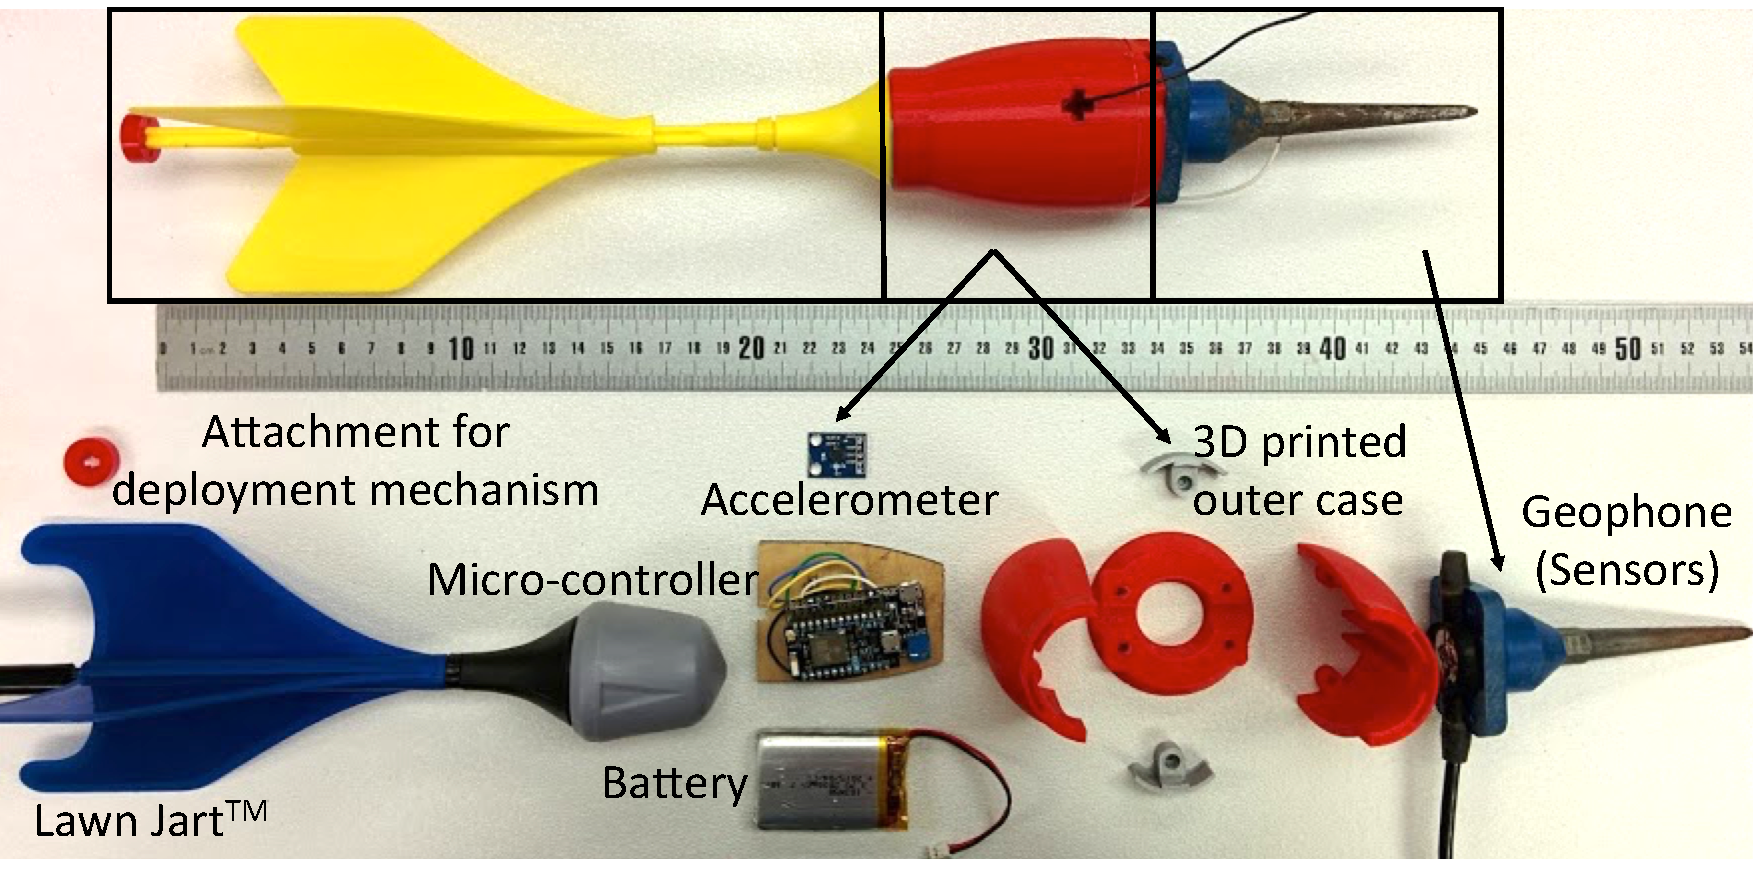
\includegraphics[width=\columnwidth]{Smart_Dart_overview.pdf}}
\caption{Cross-section of the SmartDart sensor. It consists of a lawn  Jart\textsuperscript{TM} fin, electron micro-controller, 3D printed protective casing and a geophone} 
\label{fig:Smart_Dart_overview}
\end{figure}

%%%%%%%%%%%%%%%%%%%%%%%%%%%%%%%%%%%%%%%
\subsection{Experiments}
The following sections compare SmartDart performance.
\subsubsection{ Drop tests in different soils} 
This experiment varied the drop height and measured the penetration depth in four types of soil.
Proper planting of a geophone requires (1) pushing the spike deep into the soil to ensure good contact, and (2) aligning the sensors with the gravity vector.
Each trial measured penetration depth and the angular error from vertical.

Soil types are calibrated using a hand-held penetrometer (E-280)

To determine how smart darts perform in different soils, this experiment measured penetration into four soil types. 
 Each trial was performed by holding the darts at the tip opposite to the spike in a vertical position,  releasing them at varying heights into the buckets of soil.
  measuring their penetration depth, and angle of penetration. To measure penetration depth, the buried darts were marked where the spike met the soil, the dart was then pulled from the soil, and the distance from the spike tip to the marking was measured with calipers. The angle of penetration was recorded from the accelerometer inside the dart. The soil types were categorized by their compression strength, measured using a pocket penetrometer. Measurements for compression strength vary drastically with small deviation in measurement location, so we took this measurement 10 times at 10 different locations in each soil type and took the average. A graph displaying these varying heights vs. their penetration depth can be seen in Fig.~\ref{fig:DepthPlotIndoors} and a graph displaying the penetration angle at the varying heights can be seen in Fig.\ \ref{fig:AnglePlotIndoors}

\begin{figure} \centering
{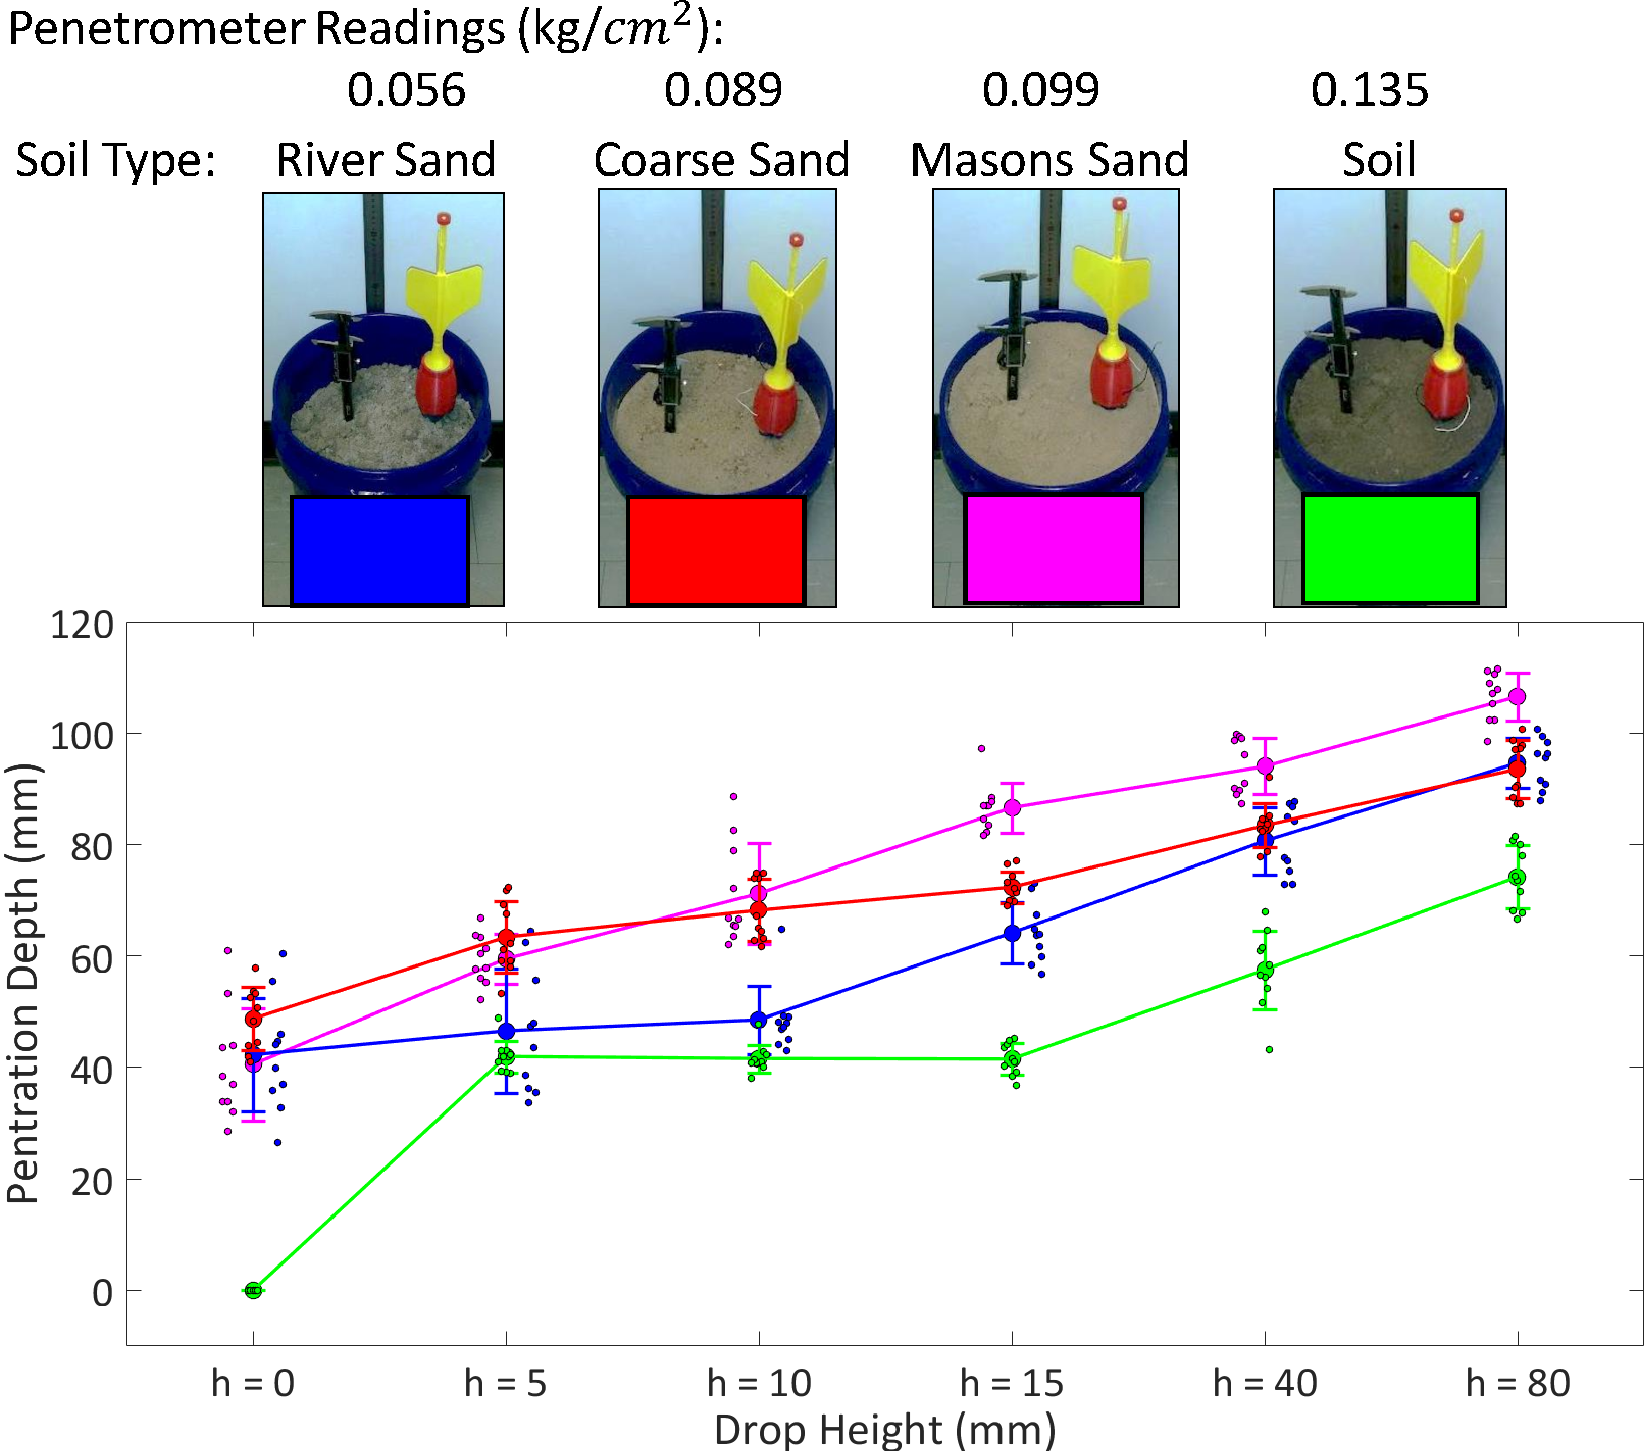
\includegraphics[width=\columnwidth]{indoor_depth_plot.pdf}}
\caption{Drop height vs. penetration depth in four soil types.} 
\label{fig:DepthPlotIndoors}
\end{figure}

\begin{figure} \centering
{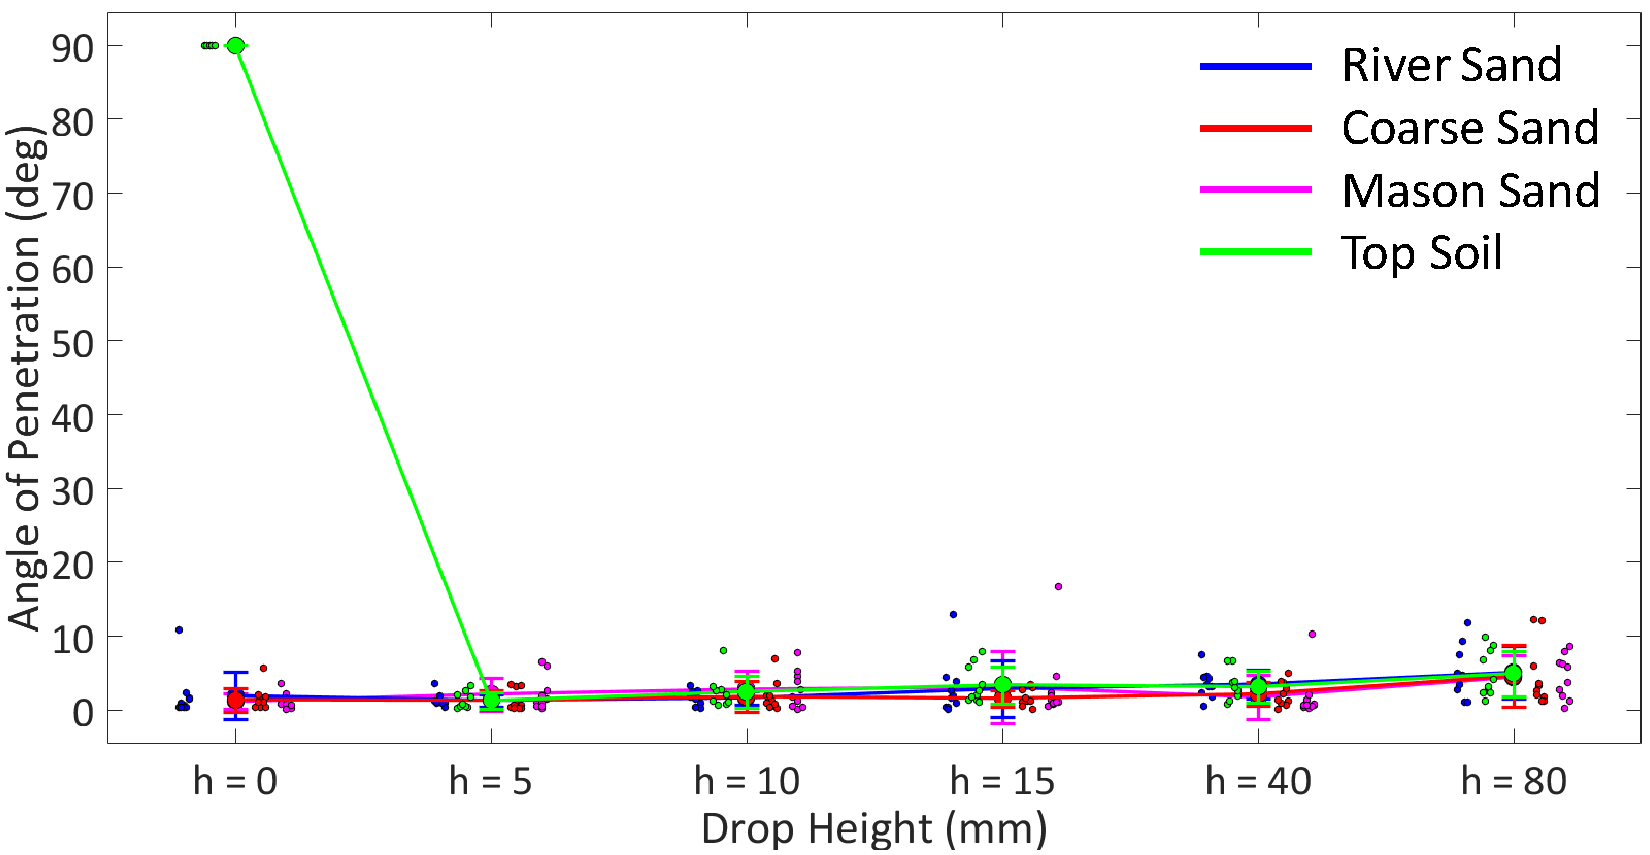
\includegraphics[width=\columnwidth]{indoor_angle_plot.pdf}}
\caption{Drop height vs. angle of deviation in four soil types.} 
\label{fig:AnglePlotIndoors}
\vspace{-1em}
\end{figure}

\subsubsection{Straight vs Bent Fins}

%Drop tests as function of height. Compares depth and angle for twisted vs. straight tail.
%Results are summarized in 

 To determine the difference in performance between straight-finned darts and twisted-finned darts, we ran a drop test with 10 trials for both types of dart at a constant height in one soil type. Each trial was initialized by holding the dart horizontally at a height of 10.5 meters, dropping it into the soil, and recording the penetration depth and penetration angle. Holding the darts horizontally emphasized the angle-correcting behavior of the fins. The angle of penetration and penetration depth were recorded as in the other drop test experiments. A graph showing the values recorded for penetration depth and angle in Fig.~\ref{fig:StraightBentPic} reveals that twisted-finned darts had greater variation in angle and less penetration.
\begin{figure} \centering
  {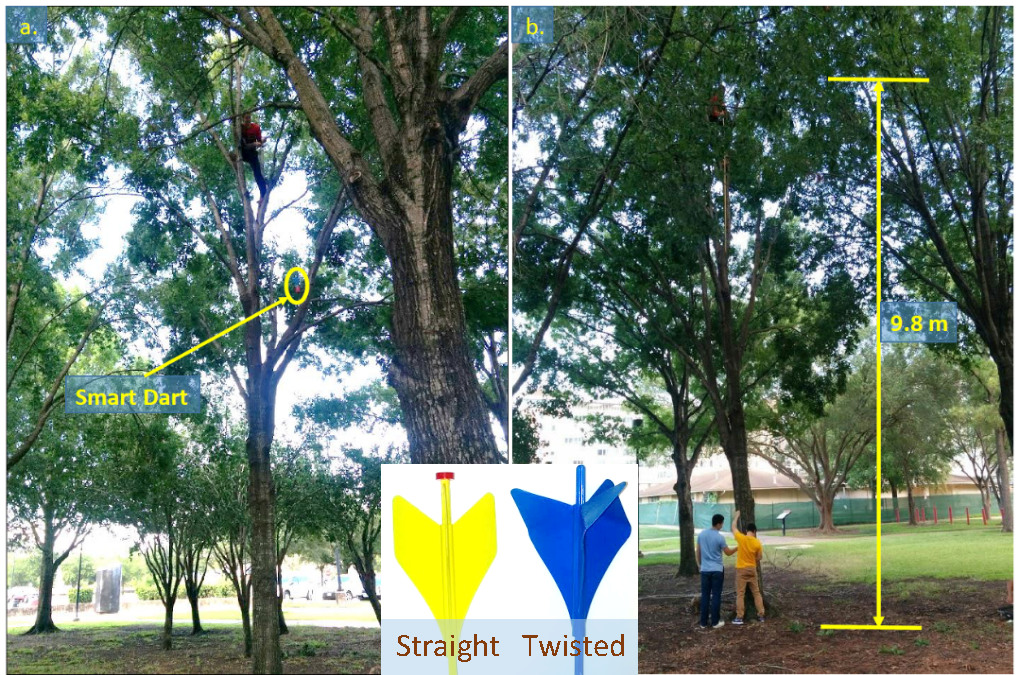
\includegraphics[width=\columnwidth]{StraightvsBent_pic.pdf}}
 \caption{Outdoor Drop test comparing Straight vs Bent fins performance.
 a.)  smart dart dropping 
 b.)  measuring drop height} 
 \label{fig:StraightBentPic}
 \vspace{-1em}
\end{figure}
\begin{figure} \centering
  {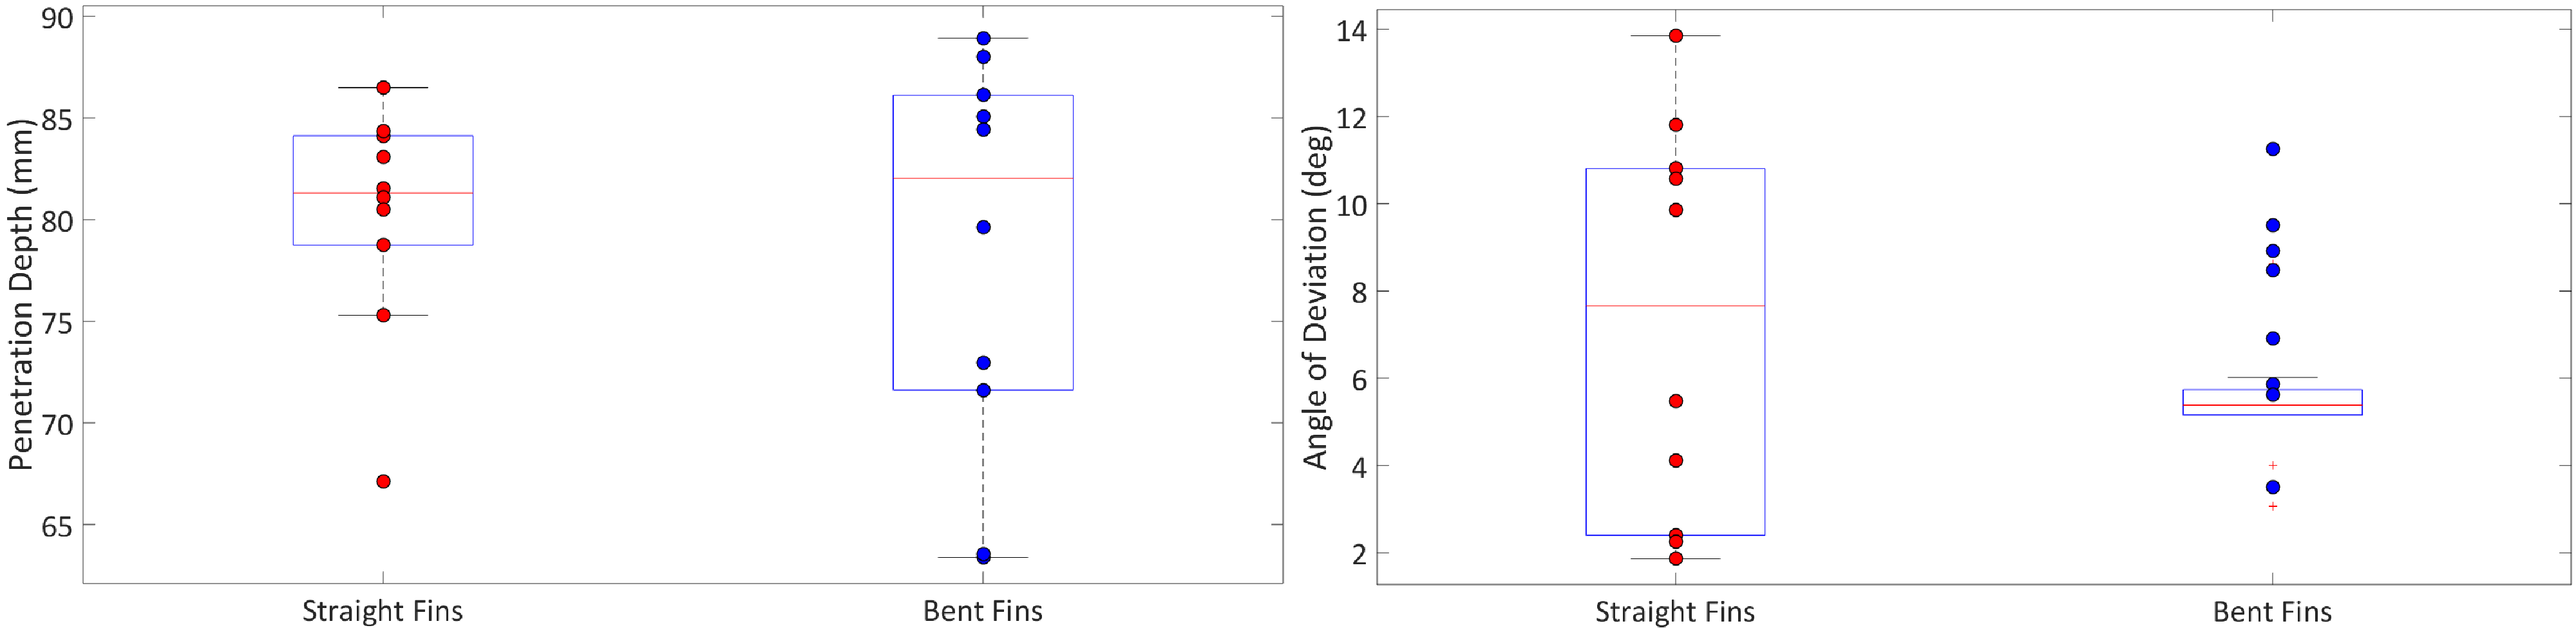
\includegraphics[width=\columnwidth]{StraightvsBent_depthangle.pdf}}
 \caption{\label{fig:StraightBentDepth}Straight vs Bent fins comparing a.) penetration depth b.) angle of deviation. Experiment used a fixed drop height of 9.8 m.} 
\end{figure}
%\begin{figure}\centering 
%\subfigure[\label{subfig:StraightBentDepth}]
%  {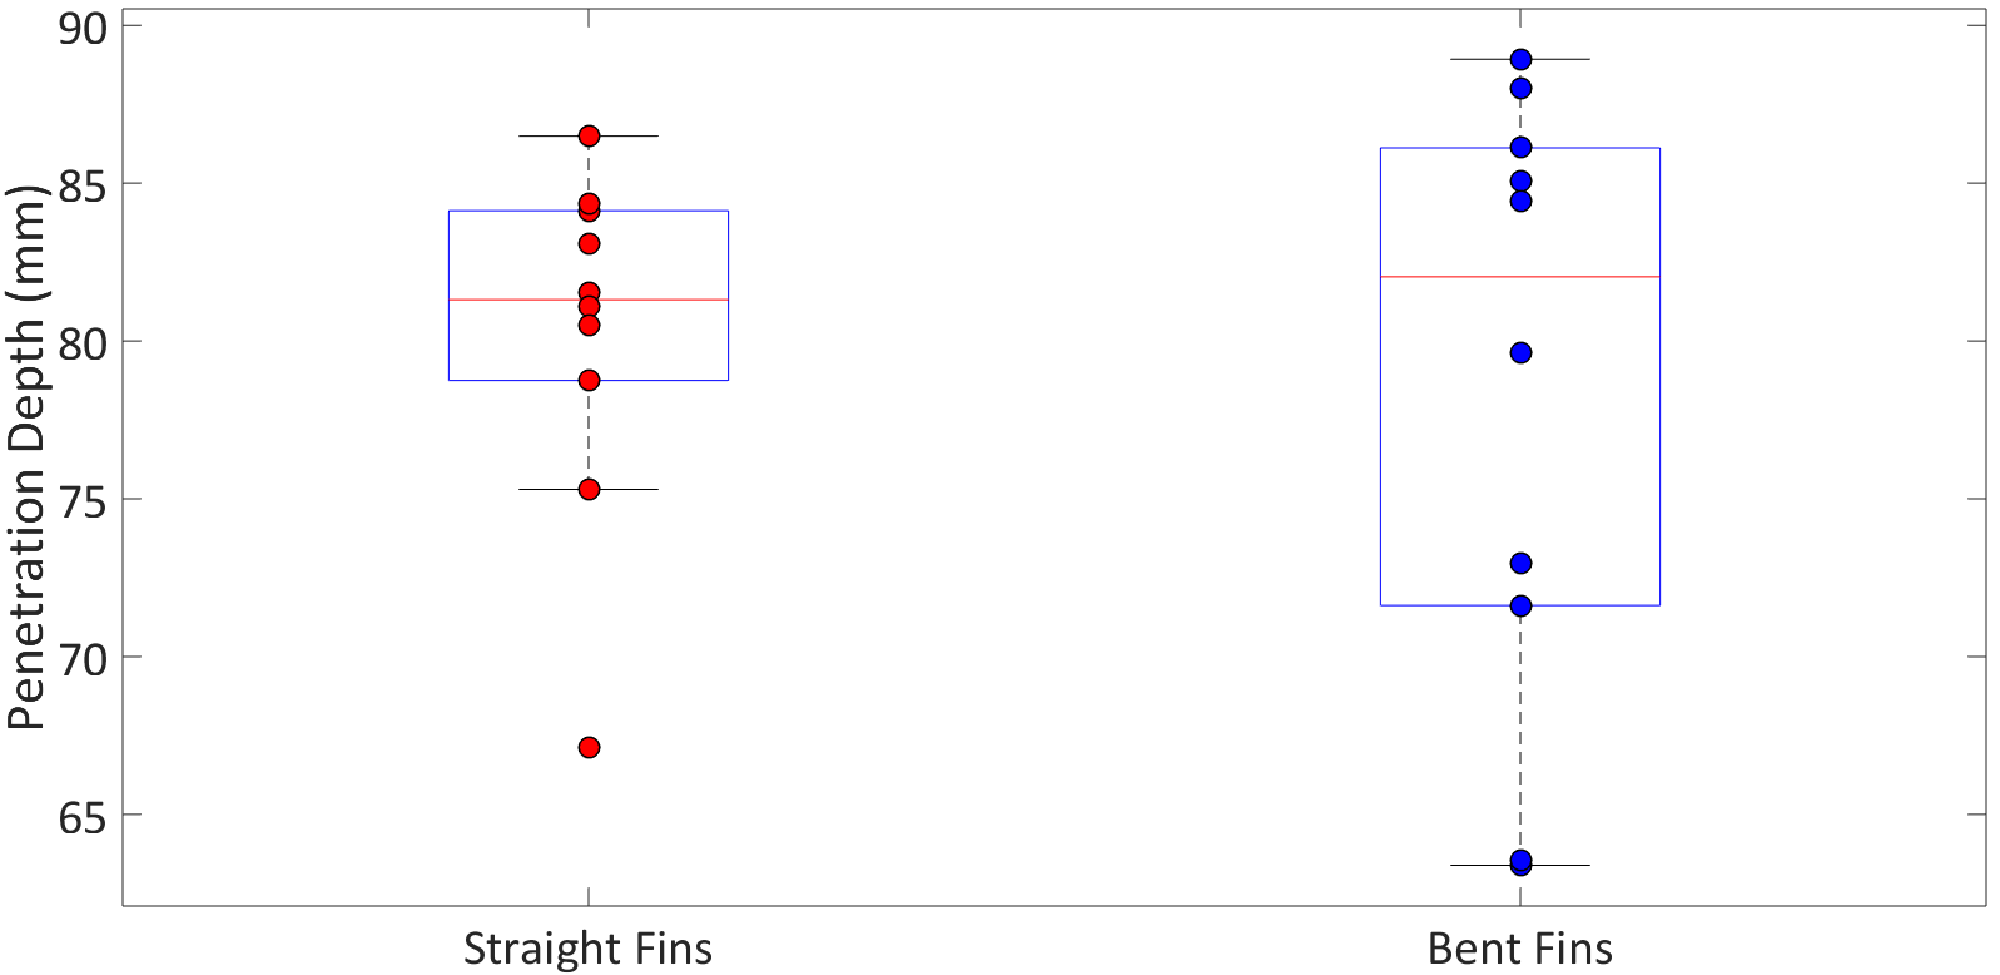
\includegraphics[width=.45\columnwidth]{StraightvsBent_depth.pdf}}
% \subfigure[\label{subfig:StraightBentAngle}]
%  {\includegraphics[width=.45\columnwidth]%{StraightvsBent_angle.pdf}}
%   \vspace*{-.1in}
 %\caption{Straight vs Bent fins comparing a.) Penetration Depth b.) Angle of Deviation. Experiment used a fixed drop height of 9.8 m. \label{fig:StraightBent}}
 %\vspace*{-.1in}
%\end{figure}
\subsubsection{Shot gather comparison}
Exp 3: Dart sensing accuracy vs ground setup

\begin{figure} \centering
  {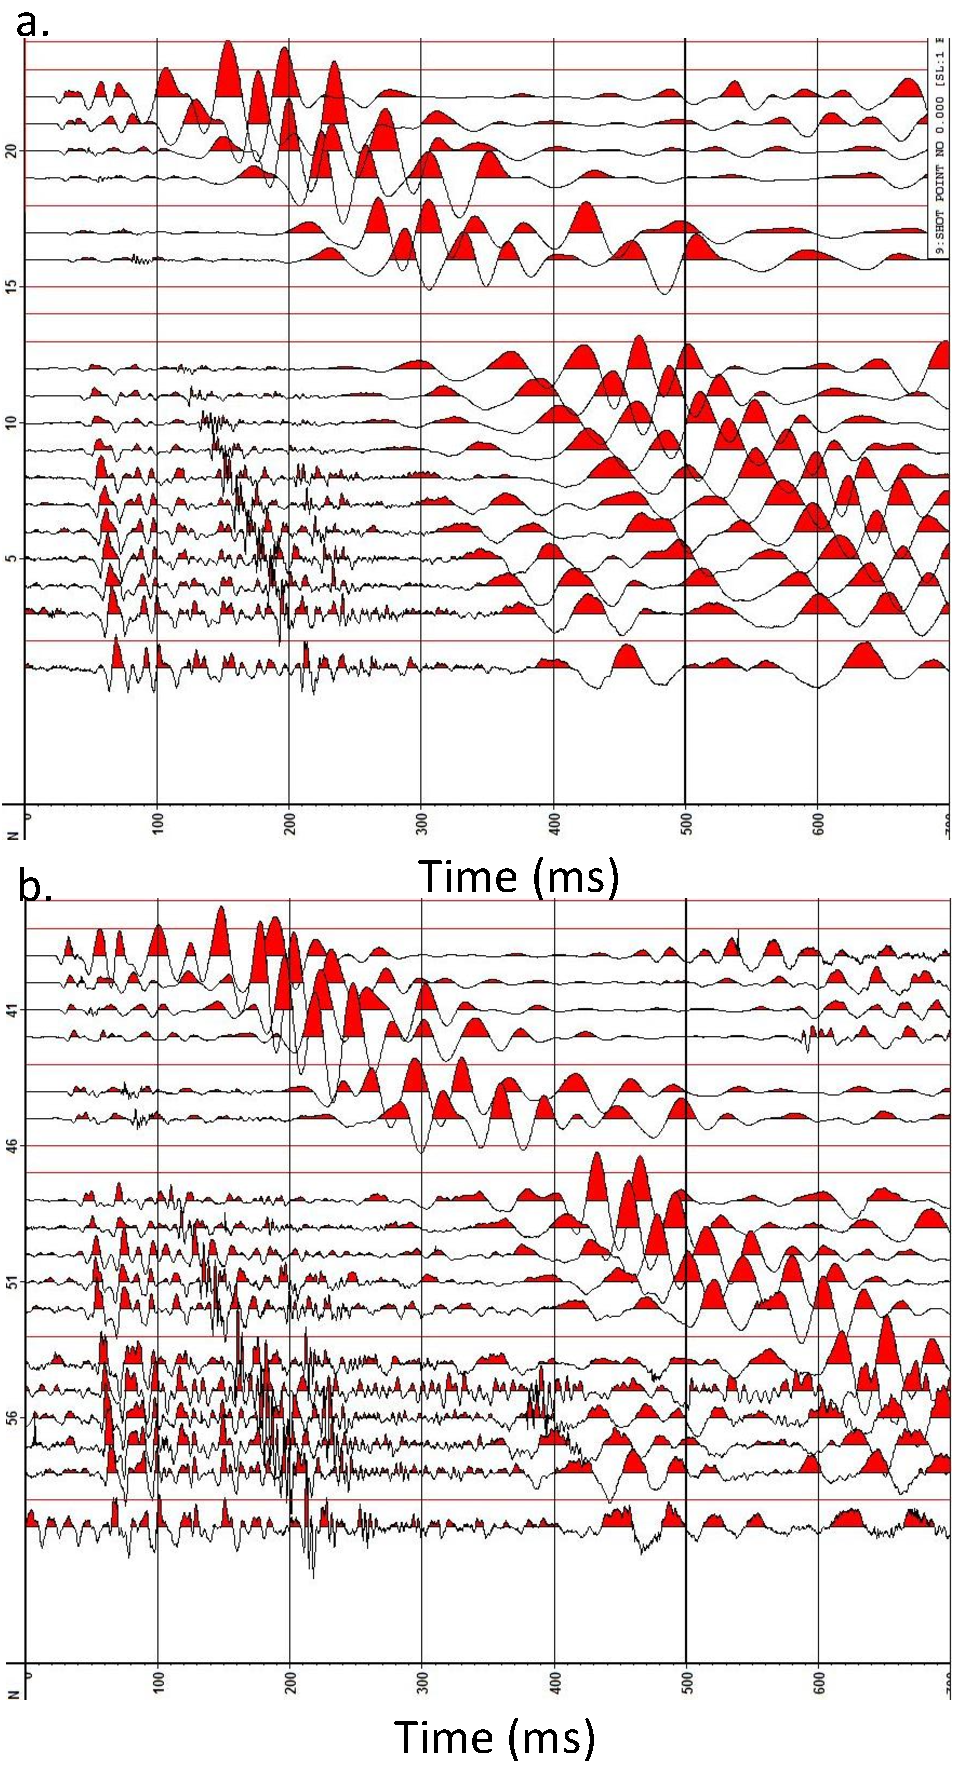
\includegraphics[width=\columnwidth]{shotgather_auto_drop.pdf}}
 \caption{Shot gather comparision of traditional geophones vs autonomously dropped smart dart sensors a.) Traditional b.) Smart darts} 
 \label{fig:TradvsAutoDrop}
\end{figure}


 